\documentclass[12pt,a4paper]{article}

\usepackage[utf8]{inputenc}
\usepackage[T2A]{fontenc}
\usepackage[ukrainian]{babel}

\usepackage{geometry}
\geometry{left=2cm,right=2cm,top=2cm,bottom=2cm}

\usepackage{graphicx}
\usepackage{array,multirow}
\usepackage{booktabs}
\usepackage{caption}
\usepackage{subcaption}
\renewcommand{\thetable}{№\arabic{table}}
\captionsetup[table]{name=Таблиця}

\usepackage{amsmath}
\usepackage{pdflscape}
\usepackage{xcolor}

\usepackage{hyperref}

\begin{document}

    \begin{titlepage}

        % Картинка шапки (по центру, з відступом від верху)
        \begin{center}
\includegraphics[width=0.7\textwidth]{../../../TITLES/letterhead.png}\end{center}

        \begin{center}
            \large Національний технічний університет України\\
            «Київський політехнічний інститут імені Ігоря Сікорського»\\[1em]
            Факультет інформатики та обчислювальної техніки\\
            Кафедра обчислювальної техніки
        \end{center}

        \vfill

        \begin{center}
            \textbf{\LARGE Практична електроніка}\\[2em]
            \textbf{\Large Лабораторна робота №2}\\[1em]
            «Дослідження операційних підсилювачів»
        \end{center}

        \vfill

        \begin{flushright}
            Виконав: студент 2 курсу ФІОТ, гр. ІО-41\\
            \textit{Давидчук А.~М.}\\[1em]
            Перевірив: \textit{Гайдай А.~Р.}
        \end{flushright}

        \vfill

        \begin{center}Київ --- 2025\end{center}

    \end{titlepage}

    % Основний документ:

    \setlength{\parindent}{0em}

    \textbf{\underline{Тема:}} «Дослідження операційних підсилювачів».
    
    \vspace{1em}

    \textbf{\underline{Мета:}} Дослідити принцип дії, основні властивості та характеристики
операційних підсилювачів (ОП). Ознайомитись із основними параметрами цих
пристроїв та областю їх застосування.

    \begin{center} \textbf{\Large Практична частина} \end{center}

    Мій порядковий номер у списку: 6. Звідси визначу, що $K = 6$.

    \begin{center} \textbf{\large Аналіз схеми №1: Схема розімкненого ОП, який не інвертує} \end{center}

    Побудуємо схему (рис. 1):

    \begin{figure}[h!]

        \renewcommand{\thefigure}{\arabic{figure}} % робимо "3.1", "3.2" і т.д.

        \centering
        % Підставляєте потрібний шлях та розмір зображення:
        
\includegraphics[width=0.5\textwidth]{scheme1.png}
        % Підпис (зазвичай під малюнком):
        \caption{\centering Схема розімкненого ОП, який не інвертує}
        % Мітка для посилань у тексті (\ref{fig:...})
        \label{scheme1}

    \end{figure}

    Далі отримаємо такі часові діаграми роботи схеми (рис. 2):

    \begin{figure}[h!]

        \renewcommand{\thefigure}{\arabic{figure}} % робимо "3.1", "3.2" і т.д.

        \centering
        % Підставляєте потрібний шлях та розмір зображення:
        
\includegraphics[width=1.0\textwidth]{graph1.png}
        % Підпис (зазвичай під малюнком):
        \caption{Часові діаграми роботи схеми (зміна вхідної та вихідної напруг)}
        % Мітка для посилань у тексті (\ref{fig:...})
        \label{graph1}

    \end{figure}

    \setlength{\parindent}{1.5em}

    З неї видно, що при вхідній напрузі $U_{\text{вх}} = -5$ В, вихідна напруга дорівнює 
    $U_{\text{вих}} = -U_{\text{нас}} = -13$ В. В момент часу $t_1$ відбувається стрибок значення вхідної
    напруги до $U_{\text{вх}} = 5$ В, а вихідна в той час: $U_{\text{вих}} = U_{\text{нас}} = 13$ В.

    \newpage

    \begin{center} \textbf{\large Аналіз схеми №2: Випробування розімкненого ОП, який інвертує} \end{center}

    \setlength{\parindent}{0em}

    Побудуємо тепер схему розімкнення ОП, який \textit{інвертує} (рис. 3):

    \begin{figure}[h!]

        \renewcommand{\thefigure}{\arabic{figure}} % робимо "3.1", "3.2" і т.д.

        \centering
        % Підставляєте потрібний шлях та розмір зображення:
        
\includegraphics[width=0.5\textwidth]{scheme2.png}
        % Підпис (зазвичай під малюнком):
        \caption{\centering Схема розімкненого ОП, який інвертує}
        % Мітка для посилань у тексті (\ref{fig:...})
        \label{scheme2}

    \end{figure}

    І наведемо часові діаграми роботи цієї схеми (рис. 4):

    \begin{figure}[h!]

        \renewcommand{\thefigure}{\arabic{figure}} % робимо "3.1", "3.2" і т.д.

        \centering
        % Підставляєте потрібний шлях та розмір зображення:
        
\includegraphics[width=1.0\textwidth]{graph2.png}
        % Підпис (зазвичай під малюнком):
        \caption{Часові діаграми роботи схеми (зміна вхідної та вихідної напруг)}
        % Мітка для посилань у тексті (\ref{fig:...})
        \label{graph2}

    \end{figure}

    \setlength{\parindent}{1.5em}

    Спочатку на вхід, який інвертує, подається напруга $U_{\text{вх}}=-5$ В, а на виході $U_{\text{вих}} = U_{\text{нас}} = 13 $ В.
    В момент часу $t_1$ відбувається стрибок значення вхідної напруги до $U_{\text{вх}} = 5$ В, а вихідна в той час: $U_{\text{вих}} = -U_{\text{нас}} = -13$ В.
    Це свідчить про інвертуючу властивість підсилення даної схеми.

    \begin{center} \textbf{\large Аналіз схеми №3: Підсилювач на базі ІМС ОП, який інвертує} \end{center}

    Мій коефіцієнт підсилення $K = 6$. Тоді на основі формули (1) коефіцієнта підсилення інвертуючого ОП:

    \[
    K_U = -\frac{R_2}{R_1}
    \tag{1}
    \]

    Поставлю, наприклад, що $R_1 = 1$ кОм, тоді $R_2 = 6$ кОм. Також відомо, що напруга насичення $U_{\text{нас}} \approx\pm13$ В. Звідси із коефіцієнтом
    підсилення $K = 6$ маємо, що при вхідній напрузі $\left|U_{\text{вх}}\right| > \frac{13}{6}$ В, значення вихідної напруги не буде перевищувати значення $\approx13$ В і на графіку буде
    спостерігатись пряма лінія в області перевищення напруги насичення.

    Для експериментальної перевірки, побудуємо два графіки: при активному (амплітуда синусусоїдного джерела $A=1$ В) та
    насиченому (амплітуда синусусоїдного джерела $A=1\cdot K=6$ В, що є досить достатньою, задля спостережень доволі помітних ліній) режимах роботи ОП.

    \begin{figure}[h!]

        \renewcommand{\thefigure}{\arabic{figure}} % робимо "3.1", "3.2" і т.д.

        \centering
        % Підставляєте потрібний шлях та розмір зображення:
        
\includegraphics[width=0.7\textwidth]{scheme3.png}
        % Підпис (зазвичай під малюнком):
        \caption{\centering Схема підсилювача на базі ІМС ОП, який інвертує}
        % Мітка для посилань у тексті (\ref{fig:...})
        \label{scheme3}

    \end{figure}

    Наведемо часові діаграми роботи схеми при активному режимі роботи ОП (рис. 6):

    \begin{figure}[h!]

        \renewcommand{\thefigure}{\arabic{figure}} % робимо "3.1", "3.2" і т.д.

        \centering
        % Підставляєте потрібний шлях та розмір зображення:
        
\includegraphics[width=1.0\textwidth]{graph3-1.png}
        % Підпис (зазвичай під малюнком):
        \caption{Часові діаграми роботи схеми, при не насиченому режимі роботи ОП}
        % Мітка для посилань у тексті (\ref{fig:...})
        \label{graph3-1}

    \end{figure}

    Тут бачимо різицю між амплітудами вхідної та вихідної напруг при активному (не насиченому) режимі роботи
    ОП. Амплітуда вихдіної напруги виявилас у приблизно 6 порядків білша, аніж вхідна, оскільки відношення
    опорів резисторів $R_2$ та $R_1$ дорівнює 6 -- це і є той коефіцієнт підсилення $K$. І також
    варто зазначити, що фаза вхідного та вихідного сигналів протилежні одна одній, що
    свідчить про інвертуючі властивості роботи ОП.

    \newpage

    Далі наведемо графік роботи при насиченому режимі роботи ОП (рис. 7):

    \begin{figure}[h!]

        \renewcommand{\thefigure}{\arabic{figure}} % робимо "3.1", "3.2" і т.д.

        \centering
        % Підставляєте потрібний шлях та розмір зображення:
        
\includegraphics[width=1.0\textwidth]{graph3-2.png}
        % Підпис (зазвичай під малюнком):
        \caption{Часові діаграми роботи схеми, при насиченому режимі роботи ОП}
        % Мітка для посилань у тексті (\ref{fig:...})
        \label{graph3-2}

    \end{figure}

    Тут можна спостерігати, що графік вихідної напруги «обрізаний»\, прямокутною формою,
    внаслідок того, що значення вихідної підсиленої напруги перевищує напругу насичення через підслення вхідної шляхом зміни амлпітуди синусусоїдного джерела:
    $U_{\text{вих}} = U_{\text{вх}} \cdot K = -6 \text{ В } \cdot 6 = -36$ В, що за модулем значно більше за $U_{\text{нас}} = 13$ В. 

    І знову ж таки, варто було лише змінити амлітуду синусусоїдного джерела більше, ніж $\frac{13}{6} - 1$ В, щоб вона набула значення
    більшого $A = \frac{13}{6}$ В, наприклад, до значення $\frac{14}{6}$ В, задля підвищення значення вхідної напруги на $K$ порядків,
    тобто щоб вихідна напруга за модулем стала $\left|U_{\text{вих}}\right| = 14$ В, що також перевищуватиме значення напруги насичення.

    \begin{center} \textbf{\large Аналіз схеми №4: Підсилювач на базі ІМС ОП, який не інвертує} \end{center}

    Мій коефіцієнт підсилення $K = 6$. Тоді на основі формули (2) коефіцієнта підсилення не інвертуючого ОП маю таку формулу $K$:

    \[
    K_U = 1+\frac{R_2}{R_1}
    \tag{2}
    \]

    Поставлю, наприклад, що $R_1 = 1$ кОм, тоді $R_2 = 5$ кОм. Також відомо, що напруга насичення $\left|U_{\text{нас}}\right| \approx13$ В. Звідси із коефіцієнтом
    підсилення $K = 6$ маємо, що при вхідній напрузі $\left|U_{\text{вх}}\right| > \frac{13}{6}$ В, значення вихідної напруги за модулем не буде перевищувати значення $\approx13$ В і на графіку буде
    спостерігатись пряма лінія в області перевищення напруги насичення.

    Для експериментальної перевірки, побудуємо два графіки: при активному (амплітуда синусусоїдного джерела $A=1$ В) та
    насиченому (амплітуда синусусоїдного джерела $A=1\cdot K=6$ В, що є досить достатньою, задля спостережень доволі помітних ліній) режимах роботи ОП.

    \newpage

    Наведемо спочатку схему (рис. 8):

    \begin{figure}[h!]

        \renewcommand{\thefigure}{\arabic{figure}} % робимо "3.1", "3.2" і т.д.

        \centering
        % Підставляєте потрібний шлях та розмір зображення:
        
\includegraphics[width=0.7\textwidth]{scheme4.png}
        % Підпис (зазвичай під малюнком):
        \caption{\centering Схема підсилювача на базі ІМС ОП, який не інвертує}
        % Мітка для посилань у тексті (\ref{fig:...})
        \label{scheme4}

    \end{figure}

    Та побудуємо часові діаграми роботи схеми при активному режимі роботи ОП (рис. 9):

    \begin{figure}[h!]

        \renewcommand{\thefigure}{\arabic{figure}} % робимо "3.1", "3.2" і т.д.

        \centering
        % Підставляєте потрібний шлях та розмір зображення:
        
\includegraphics[width=1.0\textwidth]{graph4-1.png}
        % Підпис (зазвичай під малюнком):
        \caption{Часові діаграми роботи схеми, при не насиченому режимі роботи ІМС ОП}
        % Мітка для посилань у тексті (\ref{fig:...})
        \label{graph4-1}

    \end{figure}

    Вхідний та вихідні сигнали синфазні. Коефіцієнт підсилення згідно до формули (2) дорівнює:

    \[
    K_U = 1+\frac{R_2}{R_1} = 1 + \frac{5\text{ кОм}}{1\text{ кОм}} = 6
    \]

    \newpage

    Нижче наведено графік роботи при насиченому режимі роботи ОП (рис. 10):

    \begin{figure}[h!]

        \renewcommand{\thefigure}{\arabic{figure}} % робимо "3.1", "3.2" і т.д.

        \centering
        % Підставляєте потрібний шлях та розмір зображення:
        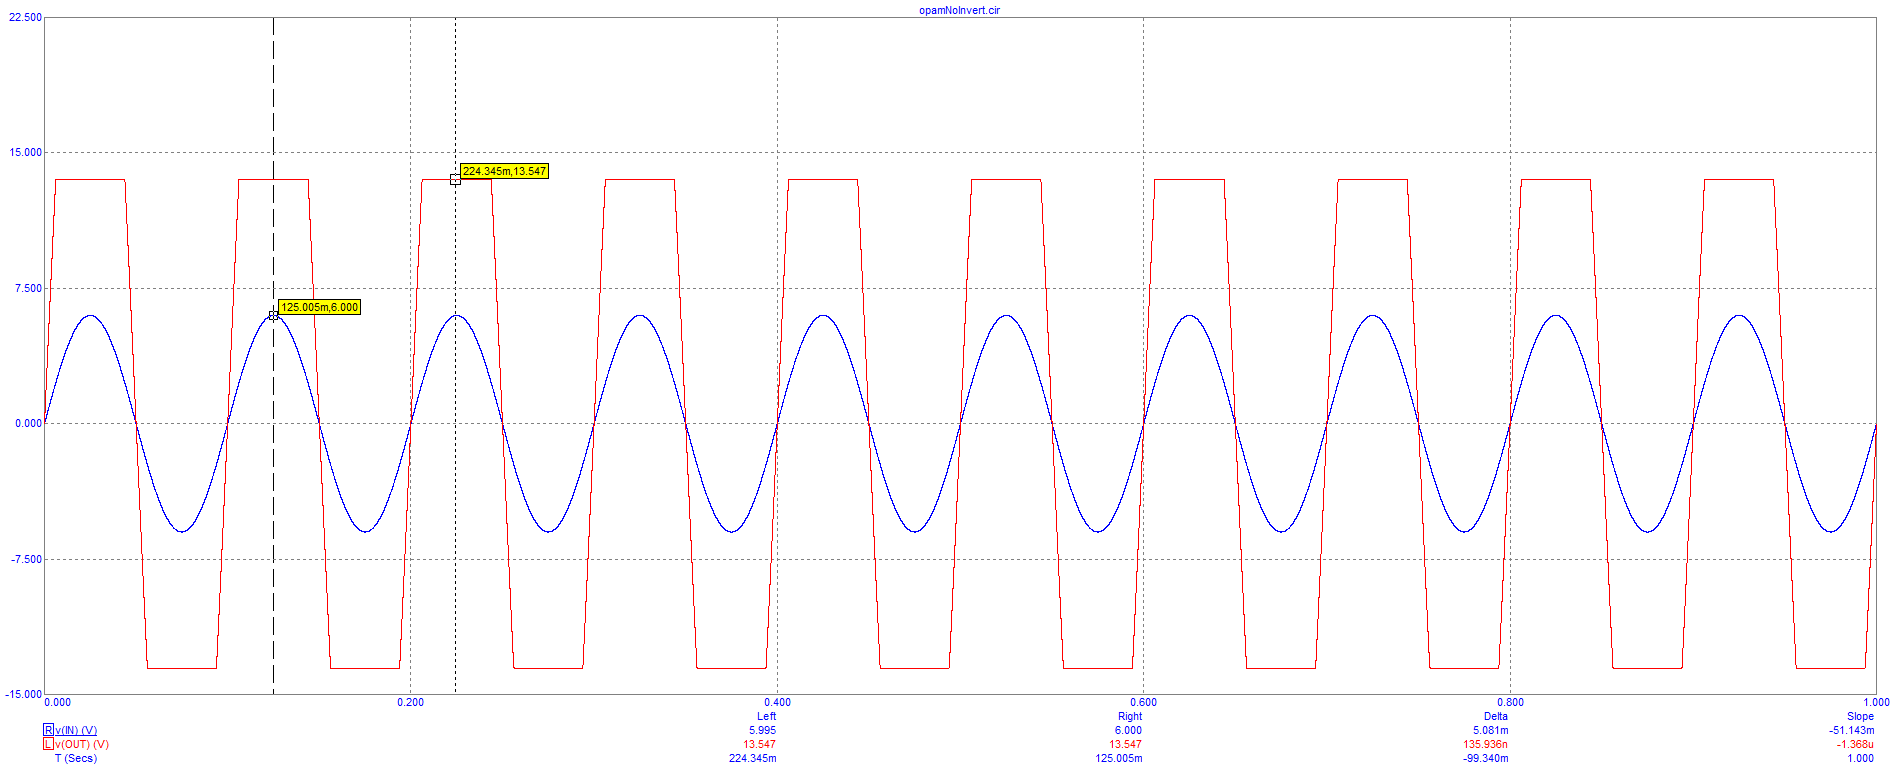
\includegraphics[width=1.0\textwidth]{graph4-2.png}
        % Підпис (зазвичай під малюнком):
        \caption{Часові діаграми роботи схеми, при не насиченому режимі роботи ІМС ОП}
        % Мітка для посилань у тексті (\ref{fig:...})
        \label{graph4-2}

    \end{figure}

    Як видно, у результаті підсилення вихідна напруга перевищила напругу 
    насичення і була «обрізана», що видно за прямокутною формою імпульсів

    \begin{center} \textbf{\large Аналіз схеми №5: Диференціюючий ланцюг на базі ІМС ОП} \end{center}

    Диференціюючий ланцюг (ДЛ) здійснює диференціювання вхідних сигналів і
    призначений для формування на виході коротких імпульсів, відповідних фронту і
    зрізу більш довгих вхідних імпульсів. ДЛ виконує фіксацію моментів фронту і зрізу
    імпульсів, що надходять на його вхід.

    Диференціюючі ланцюги виконуються з використанням або лише пасивних
    елементів (пасивні ДЛ), або з використанням пасивних та активних елементів
    (активні ДЛ). В якості частотно-залежних елементів в них можуть
    використовуватися конденсатори або індуктивності. Нижче будуть розглянуті ДЛ з
    використанням конденсаторів.

    В якості активного елементу диференціюючих ланцюгів широко
використовуються ІМС ОП.

    Нижче наведено схему активного диференціюючого ланцюга (рис. 11):

    \begin{figure}[h!]

        \renewcommand{\thefigure}{\arabic{figure}} % робимо "3.1", "3.2" і т.д.

        \centering
        % Підставляєте потрібний шлях та розмір зображення:
        
\includegraphics[width=0.5\textwidth]{scheme5-1.png}
        % Підпис (зазвичай під малюнком):
        \caption{\centering Схема активного диференціюючого ланцюга}
        % Мітка для посилань у тексті (\ref{fig:...})
        \label{scheme5-1}

    \end{figure}

    \newpage

    А також часову діаграму роботи схеми (рис. 12):

    \begin{figure}[h!]

        \renewcommand{\thefigure}{\arabic{figure}} % робимо "3.1", "3.2" і т.д.

        \centering
        % Підставляєте потрібний шлях та розмір зображення:
        
\includegraphics[width=1.0\textwidth]{graph5-1.png}
        % Підпис (зазвичай під малюнком):
        \caption{Часові діаграми роботи активного ДЛ}
        % Мітка для посилань у тексті (\ref{fig:...})
        \label{graph5-1}

    \end{figure}

    Як видно з рис. 12, вихідний сигнал має не тільки стрибок, що співпадає за
    часом зі зміною вхідного сигналу, але і коливання високої частоти. Це пояснюється
    тим, що вихідний сигнал, який за зворотним зв’язком повертається на вхід
    операційного підсилювача, збігається за фазою з вхідним сигналом. Збіг за фазою
    вхідного і вихідного сигналів виходить через зміщення на $\pi$ за рахунок
    використання інверсного входу ІМС ОП (від’ємного зворотного зв’язку) та
    зміщення на $\pi$ за рахунокфазо-частотної характеристики самої схеми ІМС ОП (за
    високих частотах утворюється транзисторами всередині ІМС ОП). Таким чином у
    сумі отримуємо $2\pi$, або 0, що еквівалентно схемі з додатним зворотним зв’язком.
    Через це характеристика супроводжуватиметься «дзвоном». Даної неприємності
    можна уникнути, використавши модифікований активний диференціюючий
    ланцюг.

    Нижче наведено схемумодифікованого диференціюючого ланцюга (рис. 13):

    \begin{figure}[h!]

        \renewcommand{\thefigure}{\arabic{figure}} % робимо "3.1", "3.2" і т.д.

        \centering
        % Підставляєте потрібний шлях та розмір зображення:
        
\includegraphics[width=0.5\textwidth]{scheme5-2.png}
        % Підпис (зазвичай під малюнком):
        \caption{\centering Схема модифікованого активного диференціюючого ланцюга}
        % Мітка для посилань у тексті (\ref{fig:...})
        \label{scheme5-2}

    \end{figure}

    Подібна модифікована схема виключає появу коливань високої частоти
    («дзвону») на виході схеми. Додаткова ємність в ланцюзі зворотного зв’язку зміщує
    за фазою зворотний сигнал на деякий додатковий кут відносно вхідного сигналу. У
    результаті на виході ми маємо майже ідеальне диференціювання вхідного сигналу.
    Ємність конденсатора зворотного зв’язку вибирається на порядок менше ємності на
    вході.

    На рис. 14 наведено часову діаграму роботи модифікованого активного диференціюючого ланцюга:

    \begin{figure}[h!]

        \renewcommand{\thefigure}{\arabic{figure}} % робимо "3.1", "3.2" і т.д.

        \centering
        % Підставляєте потрібний шлях та розмір зображення:
        
\includegraphics[width=1.0\textwidth]{graph5-2.png}
        % Підпис (зазвичай під малюнком):
        \caption{Часові діаграми роботи модифікованого активного ДЛ}
        % Мітка для посилань у тексті (\ref{fig:...})
        \label{graph5-2}

    \end{figure}

    Як видно з цієї часової діаграми, на виході з’являються по два коротких
    різнополярні імпульси, які за часом відповідають передньому та задньому фронту
    вхідних імпульсів. У цьому разі додатному фронту вхідного імпульсу відповідає
    короткий від’ємний вихідний імпульс, а від’ємному фронту вхідного імпульсу --
    короткий додатний вихідний імпульс. Зміна знаку вихідних імпульсів відносно
    знаку переднього та заднього фронтів вхідних імпульсів пояснюється тим, що в
    схемі використовується вхід ІМС ОП, який інвертує.

    \newpage

    \begin{center} \textbf{\large Аналіз схеми №6: Інтегруючий ланцюг на базі ІМС ОП} \end{center}

    Інтегруючий ланцюг (ІЛ) являє собою лінійний чотириполюсник, вихідний
    сигнал якого змінюється пропорційно інтегралу вхідного сигналу, тобто

    \[
    U_{\text{вих}} = k \cdot \int_0^t U_{\text{вх}}(t) dt
    \]

    Інтегруючі ланцюгивикористовуються в схемах формування пилкоподібної
    напруги; виділення постійної складової вхідної імпульсної послідовності; селекції
    імпульсів за тривалістю і т. ін. В якості активного елементу активних інтегруючих
    ланцюгів широко використовуються ІМС ОП.

    Нижче наведено схему активного інтегруючого ланцюга (рис. 15):

    \begin{figure}[h!]

        \renewcommand{\thefigure}{\arabic{figure}} % робимо "3.1", "3.2" і т.д.

        \centering
        % Підставляєте потрібний шлях та розмір зображення:
        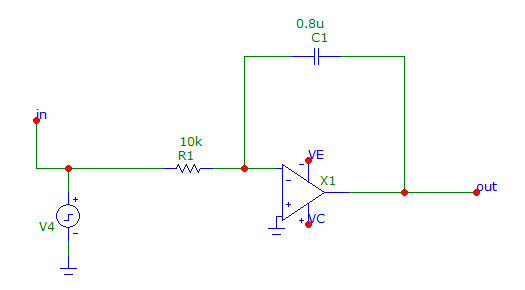
\includegraphics[width=0.7\textwidth]{scheme6.png}
        % Підпис (зазвичай під малюнком):
        \caption{\centering Схема активного інтегруючого ланцюга}
        % Мітка для посилань у тексті (\ref{fig:...})
        \label{scheme6}

    \end{figure}

    І наведемо часову діаграму роботи схеми (рис. 16):

    \begin{figure}[h!]

        \renewcommand{\thefigure}{\arabic{figure}} % робимо "3.1", "3.2" і т.д.

        \centering
        % Підставляєте потрібний шлях та розмір зображення:
        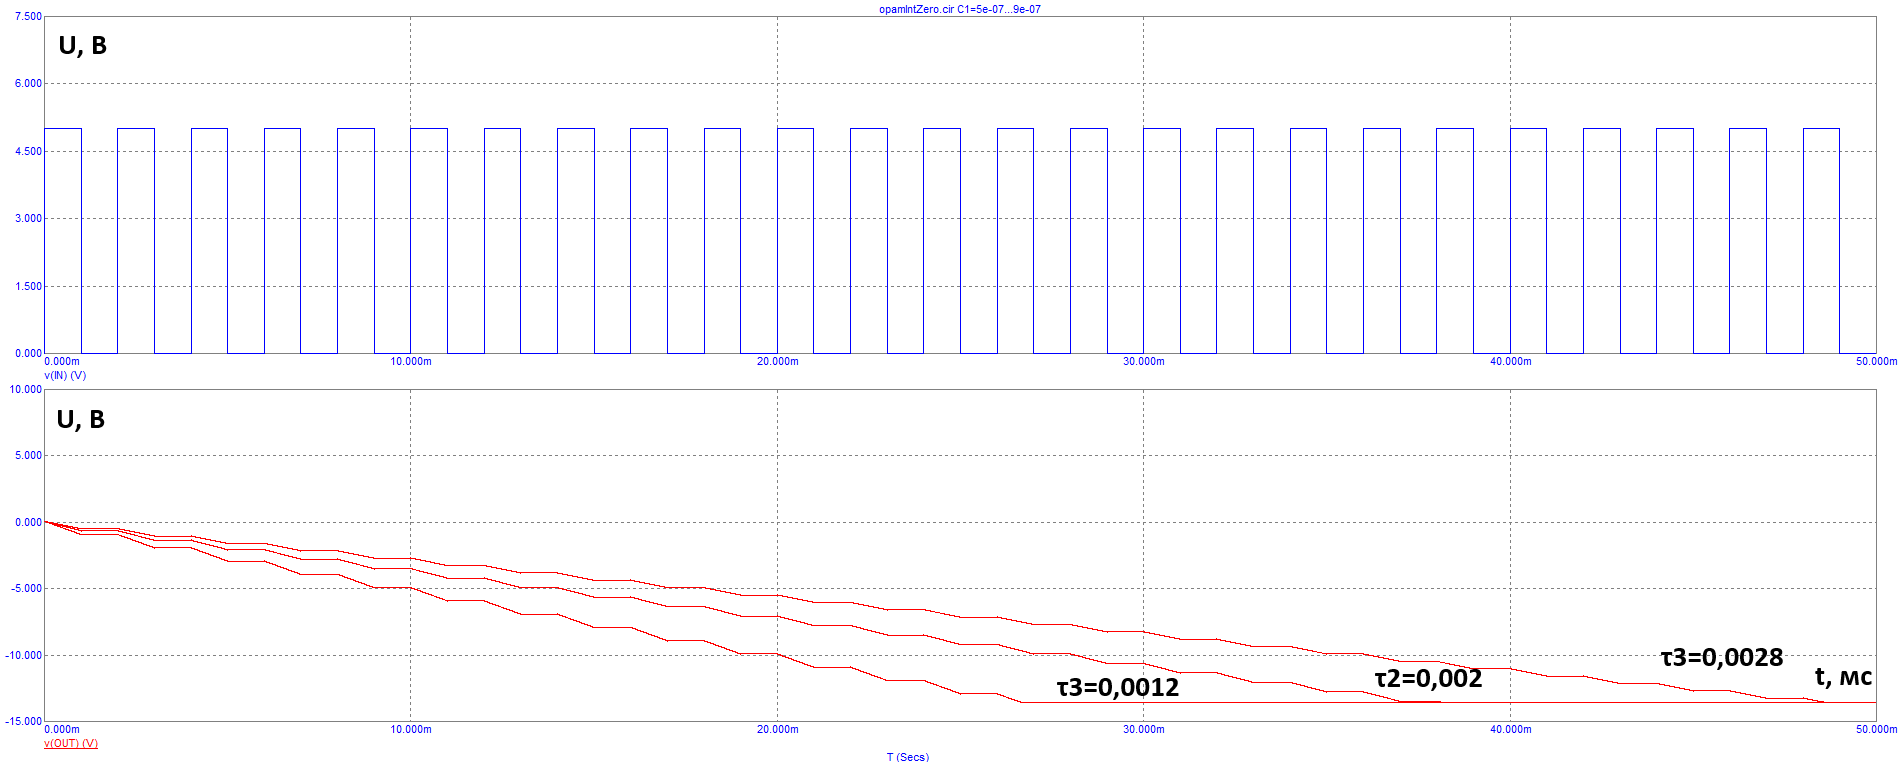
\includegraphics[width=1.0\textwidth]{graph6-1.png}
        % Підпис (зазвичай під малюнком):
        \caption{\centering Сімейство часових діаграм роботи активного ІЛ у разі зміни $R_1$ (\textit{живлення операційного підсилювача увімкнене одночасно з подачею вхідної напруги})}
        % Мітка для посилань у тексті (\ref{fig:...})
        \label{graph6-1}

    \end{figure}

    Видно, що для кожної ламаної характеристики стала часу $\tau = R \cdot C$:

    \[\tau_1 = 1500 \cdot 0{,}8u = 0{,}0012mc\]
    \[\tau_2 = 2500 \cdot 0{,}8u = 0{,}002mc\]
    \[\tau_3 = 3500 \cdot 0{,}8u = 0{,}0028mc\]

    З графіку бачимо ряд вихідних характеристик, відмінність яких одна від
    одної обумовлена різними значеннями сталої часу $\tau$. Найменший кут нахилу
    вихідної характеристики до вісі часу відповідає найбільшому значенню опору
    резистора $R_1$.

    Вихідна напруга змінюється від нуля до $-U_{\text{нас}} = -13$ B. Під час кожного
    вхідного імпульсу, амплітудою $U_m = 5$ B, вихідна напруга зменшується лінійно
    згідно з формулою

    \[
    U_{\text{вих}} = - \frac{U_m \cdot t}{RC}
    \]

    Під час кожної паузи вхідних імпульсів вихідна
    напруга не змінюється. Таким чином схема реагує на постійну складову вхідної
    імпульсної послідовності $U_{\text{сер}} = U_0$, яка має додатний знак та подається на вхід ІМС
    ОП, який інвертує.

    За рахунок $U_{\text{сер}}$ вихідна напруга поступово зменшується до рівня: $-U_{\text{нас}} = -13$ B.

    Попередньо був розглянутий випадок одночасного підключення живлення ІМС ОП і вхідної напруги.

    Якщо живлення ІМС ОПпідключити раніше, ніж подати вхідну напругу, то в
    початковий момент часу вихідна напруга буде дорівнювати: $+U_{\text{нас}}$, а потім під
    дією вхідного сигналу буде змінюватися до $-U_{\text{нас}}$.

    Нижче наведено часову діаграму роботи схеми в цьому випадку (рис. 17):

    \begin{figure}[h!]

        \renewcommand{\thefigure}{\arabic{figure}} % робимо "3.1", "3.2" і т.д.

        \centering
        % Підставляєте потрібний шлях та розмір зображення:
        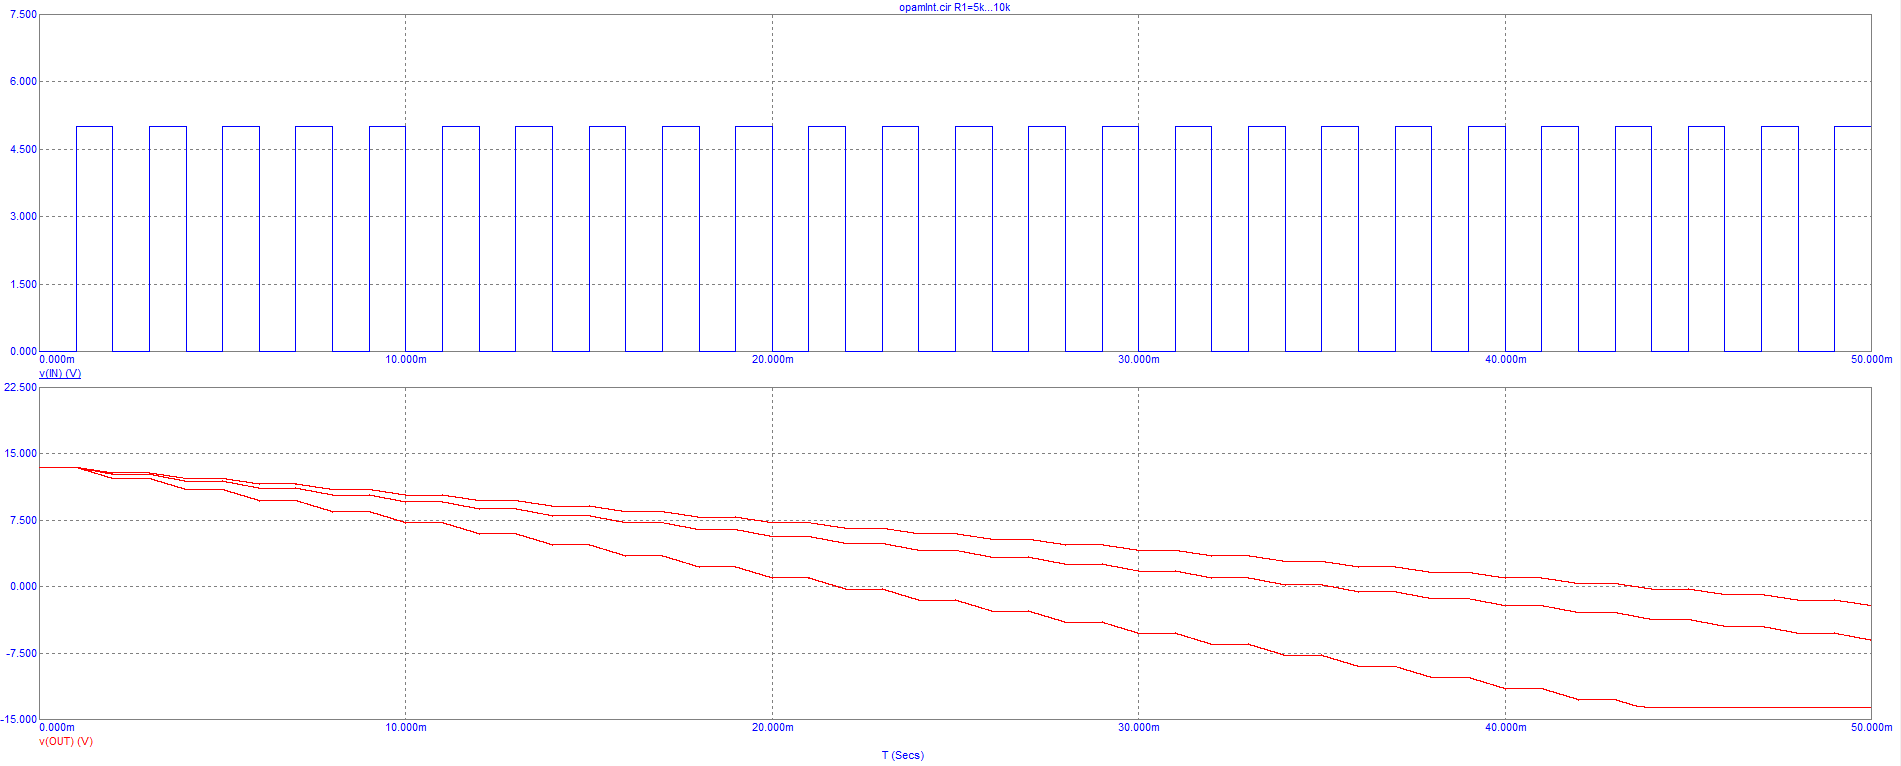
\includegraphics[width=1.0\textwidth]{graph6-2.png}
        % Підпис (зазвичай під малюнком):
        \caption{\centering Сімейство часових діаграм роботи активного ІЛ у разі зміни $R_1$ (\textit{живлення ІМС ОП увімкнене раніше, ніж подана вхідна напруга})}
        % Мітка для посилань у тексті (\ref{fig:...})
        \label{graph6-2}

    \end{figure}

    \setlength{\parindent}{0em}

    \textbf{\underline{Висновок:}} У ході лабораторної роботи досліджено принцип дії, основні характеристики та режими роботи операційних підсилювачів (ОП) у різних конфігураціях. Було розглянуто інвертуючу, неінвертуючу, диференціюючу та інтегруючу схеми, а також явища насичення, інверсії фази та вплив параметрів кола на форму вихідного сигналу.

    \setlength{\parindent}{1.5em}

Для \textbf{інвертуючого підсилювача} експериментально підтверджено формулу коефіцієнта підсилення:
\[
\displaystyle K_U = -\frac{R_2}{R_1},
\]
де знак «–» вказує на інверсію фази між вхідним і вихідним сигналами. При співвідношенні $R_2/R_1 = 6$ амплітуда вихідної напруги була у шість разів більшою за вхідну. При перевищенні вхідної амплітуди спостерігалося насичення вихідного сигналу на рівні
\[
U_{\text{нас}} \approx \pm 13~\text{В}.
\]

Для \textbf{неінвертуючого підсилювача} отримано співвідношення:
\[
\displaystyle K_U = 1 + \frac{R_2}{R_1},
\]
при якому фази вхідного та вихідного сигналів збігаються. Режим насичення проявлявся у вигляді «обрізання» вершини синусоїди.

У \textbf{диференціюючому ланцюгу} підтверджено, що вихідна напруга пропорційна похідній від вхідного сигналу:
\[
\displaystyle U_{\text{вих}} \propto \frac{dU_{\text{вх}}}{dt}.
\]
Було показано, що модифікована схема з додатковою ємністю у колі зворотного зв’язку усуває коливання («дзвін») на виході.

Для \textbf{інтегруючого ланцюга} встановлено, що вихідна напруга змінюється пропорційно інтегралу від вхідної:
\[
\displaystyle U_{\text{вих}} = k \int U_{\text{вх}}(t)\,dt,
\]
а кут нахилу характеристики залежить від сталої часу $\tau = RC$.

Отже, отримані результати повністю узгоджуються з теоретичними розрахунками та демонструють характерні властивості операційних підсилювачів у різних режимах — підсилення, інверсії, насичення, диференціювання та інтегрування.

\end{document}